\documentclass[a4paper]{report}

\usepackage{diploma}

\title{Utilisation of space-varying boundary conditions in OpenFOAM  numerical package} 

\pagestyle{main}
\begin{document}
    \placeTitlePage
    \setcounter{page}{1}
    \pagenumbering{Roman}
    \tableofcontents
    \listoffigures
    \clearpage
    \setcounter{page}{1}
    \pagenumbering{arabic}


    \chapter{Introduction}
    \section{Goal of the project}
        This work aims to achieve several goals. First one is to learn \oFoam package. 
        Get to know it's abilities and use it comfortably despite of it's rather intimidating text and console based user interface.
        Finally use it extensively for other projects since it is freely available as open source code.

        Second goal is to understand how to impose space-varying boundary conditions in \oFoam.
        In many CFD problems there is a need to impose an non uniform boundary condition, based for example on a measured data of certain quantities, in order to achieve the same conditions as in the experiment.
        One example of such situation could be validation of a simulation code or a model against collected data.
        
        
        Third goal would be to assert if conducting simulations with such boundary conditions is appropriate enough for \oFoam to be used as validation tool for various CFD models.
        In order to do that, a simple two dimensional test case will be considered and flow simulation will be performed.
        Next domain will be trimmed. Appropriate space-varying boundary conditions will be imposed on this new domain (generated from solution of the first simulation). Solution from both cases will be compared and studied.
        \begin{figure}[h]
            \centering
            \includestandalone[width=\linewidth]{Introduction/tikz/flatplate}
            \caption{Depiction of physical domains for first and second simulation with a descriptions of the boundary conditions of the original domain (including the placements of two sampling lines used for comparison of conducted simulations)}
            \label{fig::flatplate}
        \end{figure}

    \section{Description of the test case}
        In order to grasp wide spectrum of \oFoam possibilities, test case with fully turbulent flow was chosen: flow over a plat plate.
        It is a simple and very popular case, used often for turbulent model validation (the best resources describing this specific flow and an archive of validation data for turbulence models is available here~\cite{Nasa}).

        
        Simulated flow is two dimensional and incompressible (see fig. \ref{fig::flatplate}). 
        Fluid has kinematic viscosity of the air: 
        \begin{equation*}
            \nu =  \SI{1.5e-5}{\metre\squared\per\second}
        \end{equation*}
        Reynolds number $Re$ of the flow (see chapter \ref{ch::turbulence}) is equal $\num{5e6}$. Characteristic length that is used to calculate $Re$ is exactly $\SI{1}{\meter}$. 
        Knowing those parameters velocity of the fluid at the inlet can be calculated:
        \begin{equation*}
            u = \SI{75}{\metre\per\second}
        \end{equation*}
        Turbulent intensity $t_i$, at the inlet (defined as a fraction of turbulent velocity fluctuations to mean velocity value $\nicefrac{u'}{u}$) is equal to $\num{0,05}$.
        Characteristic length scale $l_T$ of those fluctuations is $\SI{1}{\meter}$.

        Second simulation will be conducted on the trimmed domain. Fields computed from the first one will be sampled along lines describing new area of calculations. Extracted data will be used to impose correct boundary conditions in the latter case. 

       
        

        
    \chapter{Theoretical background}
    \section{Turbulence and RANS equations}
        \label{ch::turbulence}
        Each flow can be characterised by a non dimensional number called the \emph{Reynolds number}:
        \begin{equation}
        Re = \dfrac{uL}{\nu}
        \end{equation}
        In the above expression symbols $u$, $L$ and $\nu$ denotes:
        \begin{itemize}
        \item[$u$] - velocity scale of the flow (e.g inlet velocity);
        \item[$L$] - characteristic length of the domain (e.g height of the step in backward facing step case);
        \item[$\nu$] - kinematic viscosity of the fluid.
        \end{itemize}
        Experiments conducted by Osborne Reynolds~\cite{Reynolds1883} prove that for low Reynolds numbers flow will remain stable even under the influence of big disturbances (e.g. separation, wall surface roughness).
        However, above certain Reynolds number each flow will lose it's laminar nature and become unstable even under the influence of very small disturbances. 
        
        Resulting oscillating flow is called turbulent. It can be described by three distinct features:
        \begin{itemize}
            \item presence of eddies and swirling motion;
            \item chaotic movement of the flow (small changes in initial conditions will cause drastic changes in flow appearance);
            \item greatly increased diffusion of any flow quantity by turbulent oscillations. 
        \end{itemize}

        Turbulence can be simulated directly. 
        Navier-Stokes equations fully describes flow of any fluid, turbulent motion included.
        Such numerical experiments are named \emph{DNS} (Direct Numerical Simulation).
        Unfortunately such approach has many disadvantages:
        \begin{itemize}
        \item in order to simulate any turbulent flow very fine mesh is necessary~\cite{Wilcox}
        \item simulation of that kind can not be simplified to a two dimensional case - turbulence is inherently a three dimensional phenomenon~\cite{landau2013fluid};
        \item DNS simulation generates a lot of data and full simulation may take days or months.
        \end{itemize}

        As of today DNS is not a viable option option for industrial CFD applications~\cite{Spalart}. Luckily there are other means to describe effects that turbulence has on fluid flow.
        In each turbulent flow two components of movement can be easily distinguished - one describing mean motion of he flow and the other corresponding to turbulent oscillations and eddies. 
        Given that, any field $\phi$ describing such flow can be decomposed into two separate fields:
        \begin{equation}
        \phi = \rans{\phi} + \phi'
        \end{equation}
        In above expression $\rans{\phi}$ denotes time averaged value~\cite{Wilcox} of $\phi$ and $\phi'$ describes turbulent fluctuations (see fig \ref{fig:RANSdecom}).

        \begin{figure}
            \centering
            \includestandalone[width = \linewidth]{Theory/tikz/rans}
            \label{fig:RANSdecom}
            \caption{Decomposition of field variable $\phi$ into time average and fluctuation part}
        \end{figure}

        In general data describing fluctuations $\phi'$ is not useful. Mean properties of the flow, on the other hand, provide much more advantageous information.
        In two similar flows, instantaneous image of two turbulent flows will be drastically different as fluctuations are chaotic in nature.
        Mean values of e.g. velocity fields will be comparable.

        In order to achieve quantitative description of fluid flow in terms of averaged variables $\rans{\bVec{u}}$ and $\rans{p}$ two operations on Navier-Stokes equations must be made:
        \begin{enumerate}
        \item Each variable must be decomposed into it's averaged and oscillating parts.
        \item Whole system of Navier-Stokes equations must be averaged in time.
        \end{enumerate}
        Having performed them, several of arising terms can be dropped and simplified resulting in \emph{Reynolds Averaged Navier-Stokes} (RANS) equations:
        \begin{equation}
        \begin{cases}
            &\pderiv{\rans{\bVec{u}}}{t} + (\rans{\bVec{u}} \cdot \nabla)\rans{\bVec{u}} = -\nabla \Big(\dfrac{\rans{p}}{\rho} \Big) %
            + \nabla\cdot \Big(\nu\nabla\rans{\bVec{u}} + \nu\nabla^T \rans{\bVec{u}} + \bm{\tau} \Big)\\
            &\nabla \cdot \rans{\bVec{u}} = 0
        \end{cases}
        \end{equation}
        The tensor $\bm{\tau}$ is called Reynolds stress tensor. It is symmetric and its components are defined in the following way:
        \begin{equation}
        \tau_{ij} = -\rans{u_i' u_j'}
        \end{equation}

        It represents effect turbulence has on the flow. Observing the above equation two remarks can be made.
        Firstly $\bm{\tau}$ is present in the exact part of equation that is "responsible" for viscous dissipation i.e. diffusion of momentum.
        It corresponds with one of the aforementioned features of turbulence: eddies increase mixing of the velocity field.
        Secondly, if Reynolds tensor is dropped from the equation original Navier-Stokes formulation is recovered.

        Unfortunately components of $\bm{\tau}$ are dependent on fluctuating parts of velocity field.
        Since no assumptions can be made about turbulent fluctuations, values of all six components of this tensor must be modelled.
        Te process of modelling components of $\bm{\tau}$ is often denoted as "closure".

        First step in closing RANS equation is assuming that Boussinesq eddy viscosity theory holds.
        It states that momentum transfer caused by turbulent eddies can be modelled by adding artificial eddy viscosity.
        Tensor $\bm{\tau}$ is then defined as:
        \begin{equation}
            \tau_{ij} =  2\nu_T S_{ij} - \dfrac{2}{3}\rans{u_\alpha' u_\alpha'}\delta_{ij} = 2\nu_T \Big(\pderiv{\rans{u}_i}{x_j} + \pderiv{\rans{u}_j}{x_i} \Big) - \dfrac{2}{3}\rans{u_\alpha' u_\alpha'}\delta_{ij}
        \end{equation}
        The last term on the right can be ignored for non-supersonic speed flows~\cite{Wilcox}.
        The newly introduced viscosity must be calculated by a chosen turbulent model.
        RANS equation after substituting Boussinesq assumption looks as follows:
        \begin{equation}
            \begin{cases}
            &\pderiv{\rans{u}_i}{t} + \rans{u}_j \pderiv{\rans{u}_i}{x_j} = -\pderiv{}{x_i}\Big(\dfrac{\rans{p}}{\rho}\Big) %
            + \pderiv{}{x_j}\Big[ (\nu + \nu_T)\Big( \pderiv{\rans{u}_i}{x_j} + \pderiv{\rans{{u}_j}}{{x_i}} \Big) \Big]\\
            &\pderiv{\rans{u}_k}{x_j} = 0
            \end{cases}
        \end{equation}

    \section{Wilcox k-$\omega$ turbulence model}
        
        In order to calculate turbulent viscosity $\nu_T$ system of two partial differential equations is introduced
        \begin{equation}
            \begin{cases}
            &\pderiv{k}{t} + \rans{u}_j \pderiv{k}{x_j} = P_k - \beta^*\omega k + %
            \pderiv{}{x_j}\Big[ (\nu + \sigma_k \dfrac{k}{\omega}) \pderiv{k}{x_j} \Big]\\
            &\pderiv{\omega}{t} + \rans{u}_j \pderiv{\omega}{x_j} = \dfrac{\gamma \omega}{k}P_k - \beta\omega^2 + %
            \pderiv{}{x_j}\Big[ (\nu + \sigma_\omega \dfrac{k}{\omega}) \pderiv{\omega}{x_j} \Big]
            \end{cases}
        \end{equation}
        First one is the equation for transport of kinetic energy of turbulent fluctuations $k$, that is defined in a following way:
        \begin{equation}
            k = \dfrac{1}{2}\rans{u'_i u'_i}
            \label{eq:k_def}
        \end{equation}
        Another scalar variable that is solved for is $\omega$ - the rate at which turbulence kinetic energy is dissipated per unit volume and time. Sometimes it is also referred to as the mean frequency of the turbulence. 
        Using those two quantities $\nu_T$ can be computed:
        \begin{equation}
            \nu_T = \dfrac{k}{\omega}
        \end{equation}


        First term on the right in the first equation is denoted as production of kinetic energy and calculated with following formula:
        \begin{equation}
            P_k = \nu_T S^2,\quad S = \sqrt{2S_{ij}S_{ij} }
        \end{equation}
        Constants present in the model have following values:
        \begin{equation*}
            \sigma_k = \sigma_\omega = 0.5,\quad \gamma = \dfrac{5}{9}
        \end{equation*}

        \begin{equation*}
            \beta = \dfrac{3}{40},\quad \beta^* = 0.09
        \end{equation*}

        In order to solve this system of equations appropriate boundary conditions must be specified. Boundary condition for $k$ can be easily deduced from it's definition (\ref{eq:k_def}):
        \begin{equation}
            k_{wall} = 0
        \end{equation}
        The same boundary condition for $\omega$ can be obtained by asymptotic analysis of the model behaviour near the solid wall~\cite{Wilcox}:
        \begin{equation}
            \omega_{wall} = \dfrac{6\nu}{\beta d_1^2}
        \end{equation}
        Variable $d_1$ is the distance from solid wall to the nearest integration point.
        Additionally inlet boundary conditions must be specified; for $k$:
        \begin{equation*}
            k_{inlet} = \dfrac{3}{2}(\vMag{\bVec{u}}t_i)^2
        \end{equation*}
        and for $\omega$:
        \begin{equation*}
            \omega{inlet} = \dfrac{\sqrt{k_{inlet}}}{l_T}
        \end{equation*}

        

    \chapter{OpenFOAM case definition}
    Case in \oFoam is defined in a very segregated way. Each piece of the case is defined in a separate text file placed in the specific directory in case directory tree (see figure \ref{fig::ofoam_folders}). 
    The most important thing to remember while editing those files is that they are essentially C++ code.
    Which means that standard C++ programming rules apply. For example each line must be ended with a semicolon. This section will describe in detail how to set up a full \oFoam case starting from mesh generation and finishing on post-processing. Input files for both cases featured in this work can be viewed and downloaded from~\cite{git}.

    \begin{figure}[h]
      
    \dirtree{%
            .1 case\DTcomment{main directory of the case}.
            .2 constant\DTcomment{constant properties of the case e.g. mesh description}.
            .2 system\DTcomment{numerical schemes, solvers and simulation settings}.
            .2 0\DTcomment{initial conditions for all fields including boundary conditions}.
            .2 100\DTcomment{solution for timestep $t=100$}.
            .2 processor*\DTcomment{part of the case that was decomposed for core "\texttt{*}"}.
    }
    \caption{Typical \oFoam case folder structure}
    \label{fig::ofoam_folders}
    \end{figure}

    \section{Turbulent flow over flat plate}
        First step in defining the case is selecting properties of transported fluid.
        This can be done by creating appropriate file in \texttt{constant} folder:
        \begin{lstlisting}[language=bash]
            mkdir constant
            touch constant/transportProperties
        \end{lstlisting}
        and editing it so it looks like this:
        \lstinputlisting[language=C++,firstline=8,lastline=40,basicstyle=\small\ttfamily]{../final_cases/NASA_fp/constant/transportProperties}

        Code starting with \lstinline[language=C++]{FoamFile} is a definition of chosen file.
        It has file's location specified and it's name. Most of the files created will be instances of \lstinline[language=C++]{dictionary} class and will have the same version and format.

        Below transport model is declared. 
        Simulated fluid has Newtonian constitutive relation.
        Next fluid kinematic viscosity is defined.
        Value $\num{1.5e-5}$ selected for this simulation is appended by description of its physical units (which is optional).
        Seven fields in braces corresponds to powers of specific SI units:
        \begin{lstlisting}[language=C++]
            [kg m s K mol A cd]
        \end{lstlisting}
        Kinematic viscosity has a unit of \si{\meter\squared\per\second} which yields \lstinline[language=C++]{[ 0 2 -1 0 0 0 0 ]} as \oFoam unit description.

        Since simulated flow is turbulent in nature, solver also needs information about turbulent modelling technique and chosen turbulence model.
        Those settings are in file named \texttt{turbulenceProperties} placed in the same folder.
        Contents of this file should look like this:
        \lstinputlisting[language=C++,firstline=8,lastline=26,basicstyle=\small\ttfamily]{../final_cases/NASA_fp/constant/turbulenceProperties}
        First \lstinline{simulationType} field must be defined. Here \lstinline{RAS} is \oFoam keyword for RANS simulation. 
        Next \lstinline{RAS} dictionary must be defined which includes choosing turbulence model, switching on the turbulence and additional options.

        \subsection{Mesh generation}
            Next step is mesh generation using \lstinline{blockMesh} utility. It is capable generating structural hexagonal meshes in three dimensions. 
            Input for \lstinline{blockMesh} is also defined in text file named \texttt{blockMeshDict} and placed in \texttt{case/system} directory. Detailed explanation and description of \lstinline{blockMesh} format is available here~\cite{blockMesh}.

            For this case \texttt{blockMeshDict} should look like this:
            \lstinputlisting[firstline=8,language=C++,basicstyle=\small\ttfamily]{../final_cases/NASA_fp/system/blockMeshDict}

            The last boundary patch is of type \lstinline{empty}. Since \oFoam can only simulate three dimensional flows. Empty boundary condition is used to reduce case to two dimensional. It should be specified in two dimensional cases on faces perpendicular to $z$ axis.

        \subsection{Defining boundary and initial conditions}
            Initial and boundary conditions must be specified for each field that is calculated during run time: $\bVec{u}$, $p$, $k$, $\omega$ and $\nu_T$.
            Every simulation in \oFoam is iterated in time (even steady ones; time is than just iteration number).
            Definitions for each of those fields is specified in the \texttt{0} folder (see figure \ref{fig::ofoam_0}) which can be interpreted as flow data from time $0$.
            \begin{figure}[b!]
      
                \dirtree{%
                        .1 case.
                        .2 0\DTcomment{initial time folder}.
                        .3 U\DTcomment{velocity field}.
                        .3 p\DTcomment{pressure field}.
                        .3 k\DTcomment{turbulent kinetic energy field}.
                        .3 omega\DTcomment{turbuelnt dissipation rate}.
                        .3 nut\DTcomment{turbulent visocsity}.
                }
                \caption{File structures defining initial and boundary conditions}
                \label{fig::ofoam_0}
            \end{figure}
            Each of the files has the same structure (and files in directories describing further times e.g. \texttt{100/U} will have the same structure as well) that can be divided into 4 sections:
            \begin{description}
                \item[\texttt{FoamFile}] - standard file description. Class of each field is defined here: \lstinline{volVectorField} is a vector field e.g. $\bVec{u}$ and \lstinline{volScalarField} is a typical scalar quantity, for example $p$.
                \item[\texttt{dimension}] - definition of physical units of the quantity.
                \item[\texttt{internalField}] - values of field variables inside the domain. In the initial time step it is connivent to use \lstinline{uniform} keyword to set one value for each cell, for example \lstinline[language=C++]{internalField   uniform (75 0 0);} initialises velocity vector with $x$ component equal to $\num{75}$.
                \item[\texttt{boundaryField}] - definitions of boundary conditions. For each \lstinline{patch} defined in \texttt{blockMeshDict} user must specify boundary condition type and value (if needed). Several of possible types are:
                \begin{description}
                    \item[\texttt{fixedValue}] - condition of Dirichlet type imposing uniform value;
                    \item[\texttt{zeroGradient}] - zero Neumann boundary condition;
                    \item[\texttt{symmetryPlane}] - condition imposing symmetry;
                    \item[\texttt{empty}] - condition placed in two dimensional cases on unnecessary patches.
                \end{description} 
            \end{description}

            
            
            Exemplary text file for velocity field is shown below:
            \lstinputlisting[language=C++, firstline=8,basicstyle=\small\ttfamily]{../final_cases/NASA_fp/0/U}
        
        \subsection{Setting up the simulation}
            In order to run any simulation a file with solver setting must be specified.
            It stores information about time step, iteration numbers and other options.
            File must be named \texttt{controlDict} and must be placed in \texttt{case/system} directory.
            
            Again it has \lstinline[language=C++]{FoamFile} field in the begging. Than it is appended by following entries:
            \begin{description}
                \item[\textbf{application}] - in this place numerical solver is specified, in this simulations \lstinline[language=C++]{simpleFoam} was chosen. It is a solver for steady turbulent problems.
                \item[\textbf{iterations}] - specification of iterations or time stepping (as here they are interchangeable) is rather self explanatory and is achieved in the following way:
                    \begin{lstlisting}[language=C++]
startFrom       startTime;
startTime       41000;
stopAt          endTime;
endTime         50000;
deltaT          1;
                    \end{lstlisting}
                \item[\textbf{saving solutions}] - there are several options for saving solutions while the simulation is running. Again they are mostly self explanatory:
                \begin{lstlisting}[language=C++]
writeControl    timeStep;
writeInterval   2000;
purgeWrite      0;
                \end{lstlisting}
                The last entry in the above list describes when solutions from previous time steps should be deleted (integer specified in \lstinline[language=C++]{purgeRight} field describes maximal number of time directories; \lstinline[language=C++]{0} means no overwriting, each solution is saved).
                \item[\textbf{I/O options}] - fields describing writing precisions for fields and time:
                \begin{lstlisting}[language=C++]
writeFormat     ascii;
writePrecision  8;
writeCompression off;                    
timeFormat      general;                 
timePrecision   8;
runTimeModifiable true;
                \end{lstlisting}
                Last entry in the above list enables altering case files during simulation time i.e.\ changing of postprocessing settings, time step etc.
            \end{description}
            In depth description of options available in \texttt{controlDict} can be found in~\cite{controlDict}.
        \subsection{Selecting numerical schemes}
            Each differential operator is in any equation must be simplified into its discrete form in order to solve such problem. Description of numerical schemes used to represent those operators is in the file \texttt{case/system/fvSchemes}.

            Another reason behind \oFoam being noticeably harder to use than other software packages that are available because is, it does not specify any standard numerical schemes for a chosen problem.
            User must specify a discrete scheme for each differential operator manually.
            For example time derivative can be defined in the following way:
            \begin{lstlisting}[language=C++]
ddtSchemes
{
    default steadyState; //default scheme (used for every field variable)
    ddt(k)  backward;    //scheme for k equation (overrides default scheme)
}
            \end{lstlisting}
            If simulation requires calculation of wall distance $y$ that method should also be specified here:
            \begin{lstlisting}[language=C++]
wallDist
{
    method          meshWave;
}
            \end{lstlisting}
            Additional documentation about numerical schemes can be found here~\cite{fvSchemes}.
        \subsection{Setting up the linear solvers}
            After the discretisation each equation is represented by system of linear equations, that is solved iteratively. User can specify a solver type and its parameters inside \texttt{case/system/fvSolution}. Since \texttt{simpleFoam} is a segregated solver (it solves for each component of $\bm{u}$ and $p$ separately) user must specify one solver for components velocity and the other one for pressure. Another two solvers for turbulent variables are also necessary. For example settings for $p$ may look like this:
            \begin{lstlisting}[language=C++]
p
{
    solver          GAMG;           //type of the solver
    tolerance       1e-16;          //final tolerance of the residual
    relTol          0.001;          //relative tolerance of the residual
    maxIter         1000;           //maximum number of iterations
    smoother        GaussSeidel;    //type of smoother
    nPreSweeps      1;              //-----------------------------
    nPostSweeps     3;              //
    nFinestSweeps   1;              //
    cacheAgglomeration on;          //settings for GAMG solver
    agglomerator    faceAreaPair;   //
    nCellsInCoarsestLevel 128;      //
    mergeLevels     1;              //-----------------------------
}
            \end{lstlisting}
            Fields \lstinline[language=C++]{tolearnce}, \lstinline[language=C++]{relTol} and \lstinline[language=C++]{maxIter} are stop criteria - when solver reaches any of those it will stop iterating. The other fields are options for chosen solver.
            
            In the same file settings for SIMPLE algorithm implemented in \texttt{simpleFoam} are placed:
            \begin{lstlisting}[language=C++]
SIMPLE
{
    nNonOrthogonalCorrectors 0; //specifies repeated solutions of the 
                                //pressure equation, used to update the
                                //explicit non-orthogonal correction

    residualControl             //stopping criteria for the algorithm 
    {                           //based on residual
        p               1e-8;
        U               1e-8;
        "(k|epsilon|omega)" 1e-8; //one criterion for multiple fields
    }
}
            \end{lstlisting}
            One setting or solver can be applied on all the fields at once, by using parenthesis and ''or'' operator (''\texttt{|}'') as seen in above example. 
            
            Another very important simulation parameter is also specified here - under-relaxation coefficients. User can specify a value for each of the variables:
            \begin{lstlisting}[language=C++]
relaxationFactors
{
    equations
    {
        U               0.5;
        p               0.3;
        k               0.5;
        omega           0.5;
    }
}
            \end{lstlisting}
            More in depth documentation of \texttt{fvSolution} file can be found here~\cite{fvSolution}.
        \subsection{Mesh decomposition}
            As in most CFD codes in \oFoam mesh can be decomposed into many parts in order to enable palatalisation of necessary calculations.
            It is achieved by creating file named \texttt{decomposeParDict} in \texttt{system} directory and running \texttt{decomposePar} utility. Insides of this file describes how mesh should be divided:
            \lstinputlisting[language=C++, firstline=8,basicstyle=\small\ttfamily]{../final_cases/NASA_fp/system/decomposeParDict}
            After parallel calculations are completed mesh and saved results can be recombined to original state by calling \texttt{reconstructPar}
        \subsection{Running the solver}
            After mesh is generated, initial and boundary conditions imposed and simulation settings set up, a solver can be run. It is achieved by using \texttt{simpleFoam} command. It will run SIMPLE segregated solver along with appropriate solvers for chosen turbulence models in serial mode (on one computation core).

            Calculations can be run in parallel mode using MPI. In order to do that first host file must be created. In case of running solver on one computer with 2 cores it should look like this:
            \lstinputlisting{../final_cases/NASA_fp/machines}
            Than solver is called with following command:
            \begin{lstlisting}
mpirun --hostfile <path to host file> -np 2 simpleFoam -parallel 
            \end{lstlisting}
            It is often useful to redirect output from \texttt{simpleFoam} to log file and run it in the background by appending above command with:
            \begin{lstlisting}
> <name of log file> & 
            \end{lstlisting}
        \subsection{Understanding and plotting the residuals}
            Example output from \texttt{simpleFoam} solver can look in the following way:
            \begin{lstlisting}[basicstyle=\footnotesize\ttfamily]
Time = 5006

smoothSolver:
Solving for Ux, Initial residual = 2.539e-05, Final residual = 1.787e-07, No Iterations 4
smoothSolver:  
Solving for Uy, Initial residual = 3.608e-05, Final residual = 2.802e-07, No Iterations 3
GAMG:
Solving for p, Initial residual = 5.525e-05, Final residual = 5.510e-10, No Iterations 586
time step continuity errors: 
sum local = 2.544e-09, global = -1.575e-10, cumulative = -6.343e-10
DILUPBiCGStab:
Solving for omega, Initial residual = 3.645e-09, Final residual = 9.800e-17, No Iterations 3
smoothSolver:
Solving for k, Initial residual = 1.321e-05, Final residual = 7.552e-17, No Iterations 21
ExecutionTime = 11.74 s  ClockTime = 12 s             
            \end{lstlisting}

            Algorithm outputs two residual values for each variable:
            \begin{description}
                \item[Initial residual] - measure of how well old solution fits new system of algebraic equations.
                \item[Final residual] - measure of convergence of linear solver. 
            \end{description}
            The first one is, at the same time, a measure of convergence of solution of nonlinear partial differential equation.
            
            In order to monitor solution convergence, plot of initial residuals against number of iterations is often useful. It can be achieved by using \texttt{gnuplot}:
            \begin{lstlisting}
gnuplot residuals
            \end{lstlisting}
            File \texttt{residuals} is a bash script\footnote{Courtesy of user \textit{wolle1982} of \url{www.cfd-online.com} forum~\cite{residuals}.} reading residual data from file named \texttt{log}:
            \begin{lstlisting}[showstringspaces=false,language=bash, basicstyle=\footnotesize\ttfamily]
set logscale y
set title "Residuals"
set ylabel 'Residual'
set xlabel 'Iteration'
plot "< cat log | grep 'Solving for Ux' | cut -d' ' -f9 | tr -d ','" title 'Ux' with lines,\
"< cat log | grep 'Solving for Uy' | cut -d' ' -f9 | tr -d ','" title 'Uy' with lines,\
"< cat log | grep 'Solving for Uz' | cut -d' ' -f9 | tr -d ','" title 'Uz' with lines,\
"< cat log | grep 'Solving for omega' | cut -d' ' -f9 | tr -d ','" title 'omega' with lines,\
"< cat log | grep 'Solving for k' | cut -d' ' -f9 | tr -d ','" title 'k' with lines,\
"< cat log | grep 'Solving for p' | cut -d' ' -f9 | tr -d ','" title 'p' with lines
pause 1
reread
            \end{lstlisting}
            It can be called while the simulation is running in the background and solver's output is redirected to a file.
        \subsection{Postprocessing}
            \oFoam has many postprocessing tools built in e.g.\ an utility used to calculate $y^+$ value in cells adjacent to viscous walls.
            Postprocessing routines can be used in three ways:
            \begin{enumerate}
                \item after the simulation - using \texttt{postProcess} command
                \item after the simulation - running chosen solver with \texttt{-postProcess} option
                \item during run time
            \end{enumerate}
            The first option is the simplest. In order to calculate any field variable, for example Courant number or $y^+$ user must call:
            \begin{lstlisting}[language=bash]
postProcess -func <field name> 
            \end{lstlisting}
            List of fields that can be calculated can be found by typing:
            \begin{lstlisting}[language=bash]
postProcess -list
            \end{lstlisting}
            For vorticity field, appropriate command will look like this:
            \begin{lstlisting}[language=bash]
postProcess -func vorticity
            \end{lstlisting}
            Program that is executed will calculate values of chosen field in each time step directory.

            Another option is to include postprocessing tools inside \texttt{controlDict} file. It is useful in situations when postprocessing requires some additional code i.e. turbulence model as in the case of wall shear stress calculation.
            In order to do that user can append \texttt{controlDict} with the following code:
            \begin{lstlisting}[language=C++]
functions
{
    #includeFunc "wallShearStress"
}
            \end{lstlisting}
            Any function that is listed here will be evaluated during run time (evaluation time is selected by \texttt{writeControl} option) and its outcome will be saved in appropriate time step directory.
            Functions can be also evaluated after simulation using \texttt{<chosen solver> -postProcess} command (more information about postprocessing and available utilities can be found here~\cite{postProc}).
        
            Postprocessing can also be done in third party software \textbf{ParaView}. It is shipped with most of \oFoam distributions and can be lunched by calling \texttt{paraFoam} utility inside case directory.
        
        \subsection{Sampling simulation data}
            Various kinds of data, for example components of velocity field, can be extracted along specified line or surface. It is achieved by introducing a new line in \lstinline[language=C++]|functions{...}| block in \texttt{controlDict} file:
            \begin{lstlisting}[language=C++]
#includeFunc "sample"
            \end{lstlisting}
            Next new file \texttt{case/system/sample} must be created with definitions of sampling surfaces. There are many options available. In case of this two dimensional simulation only extracting data along line is necessary (as seen in figure \ref{fig::flatplate}). Example \texttt{sample} file can look like this:
            \begin{lstlisting}[language=C++]
libs            ("libsampling.so"); //inclusion of executable library
type            sets;               //sets means sampling along lines
writeControl    writeTime;          
interpolationScheme cellPoint;      //selection of interpolation scheme
setFormat       raw;                //output data format
sets                                //set definitions
(
    plateHorizontal           //first set, defined as a line  
    {                         //to end with 1000 points
        type    face;
        axis    xyz;                //specifying what coordinates 
                                    //should be outputted
        start   (0.1 0.2 0);
        end     (2 0.4 0);
        nPoints 1000;
    }

    plateBegin                      //second set defined as cloud of points
    {
        type    cloud;
        axis    xyz;
        points ( #include "points" ); //inclusion of file 
                                      //with points definitions
    }
);

fields          (p U k omega);      //selection of fields to be sampled
            \end{lstlisting}
            As dictionary files are essentially a code in C++ when non uniform spacing is needed a claud of points can be simply ''pasted'' into \texttt{sample} file using standard \lstinline[language=C++]{#include} preprocessor directive.
            Data in \texttt{case/system/points} files should has following format:
            \begin{lstlisting}[language=C++]
(x1 y1 z1)  //standard openFOAM vectors, not separated by any delimiter
(x2 y2 z2)
            \end{lstlisting}
            More in detail description of sampling abilities of \oFoam can be found~\cite{sampl}
    \section{Trimmed domain - case setup}
        Trimmed domain has four distinct boundaries (see figure \ref{fig::flatplate}):
        \begin{description}
            \item[A-B]: horizontal inlet boundary that is situated \SI{0,1}{\metre} from the start of the plate.
                Velocity profile should vary across this boundary.
            \item[B-C]: skew boundary above plate surface. Velocity field is also not uniform on this boundary.
            \item[C-D]: domain outlet.
            \item[D-A]: plate surface modelled as viscous wall.   
        \end{description}
        
        Boundary conditions on edges \textbf{C-D} and \textbf{D-C} are straight forward and set up in the same way as in previous case. In order to set appropriate velocity profiles on rest of boundaries \texttt{timeVaryingMappedFixedValue} type of boundary condition has been used.
        \subsection{Velocity and turbulent fields BCs - \texttt{timeVaryingMappedFixedValue}}
            In order to use \texttt{timeVaryingMappedFixedValue} type, first correct boundary condition should be defined in \texttt{0/U} file in following manner:
            \begin{lstlisting}[language=C++]
inlet
{
    type            timeVaryingMappedFixedValue;
    offset          (0 0 0);    //offset for three dimensional vector field
    setAverage      off;        //scale field to have an certain 
                                //average value
}
            \end{lstlisting}
            As name suggests this type of boundary condition lets user to specify fields that are both changing in time and space.
            It is achieved by creating a directory named the same as chosen patch (in this case it was \texttt{inlet}) in \texttt{constant/boundaryData} directory.
            Files inside this folder have similar structure as definitions of boundary conditions in \texttt{case} directory (see figure \ref{fig::ofoam_timeVar}). For each chosen time step patch field values must be defined along with interpolation points (that are time invariant). If only initial time is specified boundary conditions will not change in time.
            \begin{figure}[ht!]
      
                \dirtree{%
                        .1 case.
                        .2 constant\DTcomment{constants folder}.
                        .3 boundaryData\DTcomment{data for \texttt{timeVaryingMappedFixedValue} boundary condition}.
                        .4 inlet\DTcomment{file with space varying data for inlet patch}.
                        .5 points.\DTcomment{file describing points where sampling was made}.
                        .5 0\DTcomment{initial time step}.
                        .6 U\DTcomment{velocity field}.
                        .6 k\DTcomment{turbulent kinetic energy field}.
                        .6 omega\DTcomment{turbulent dissipation rate}.
                        .5 <\textit{some other time step}>.       
                        .4 <\textit{name of other patch}>.             
                }
                \caption{File structures defining \texttt{timeVaryingMappedFixedValue} conditions}
                \label{fig::ofoam_timeVar}
            \end{figure}

            In order to define points and values of fields in those points sampling along lines were used.
            In this case flow is two dimensional. Having in mind that \oFoam is a three dimensional solver, it is better to provide tho sets of points for each patch - laying on both of \texttt{empty} planes\footnote{It can be achieved for example by copying and processing sampled data in a simple Matlab script.}. It will ensure that values are interpolated correctly across the "empty" dimension. File with points definition should look in the following way:
            \begin{lstlisting}[language=C++]
4 //number of points
(
(1.0000000000e-01 0.0000000000e+00 0.0000000000e+00) //coordinates
(1.0000000000e-01 2.0000000000e-06 0.0000000000e+00)
(1.0000000000e-01 4.4430910000e-06 0.0000000000e+00)
(1.0000000000e-01 7.4274379000e-06 0.0000000000e+00)
)
            \end{lstlisting}
            Velocity field file \texttt{U} is very similar in structure:
            \begin{lstlisting}[language=C++]
4 //number of points
(
(0.0000000000e+00 0.0000000000e+00 0.0000000000e+00) //vector components
(1.5774773000e+00 2.9655442000e-06 0.0000000000e+00)
(3.5008039000e+00 1.4358657000e-05 0.0000000000e+00)
(5.8499814000e+00 4.0020820000e-05 0.0000000000e+00)
)
            \end{lstlisting}

        \subsection{Pressure boundary conditions}
            A careful reader might have noticed that \oFoam is somewhat contradictory in one place. Providing boundary conditions for both pressure and velocity at the inlet to the domain is necessary.
            If those boundary conditions are not exactly complementary, it can be seen as overdetermining the Navier-Stokes equations.

            In the first of described cases this problem can be easily avoided since both zero Neumann condition for pressure and uniform velocity value are correct boundary conditions. Unfortunately neither \textbf{A-B}, nor \textbf{B-C} boundaries are defined along streamlines, and velocity field is not uniform in their vicinity, which means that zero Neumann boundary condition for pressure cannot be applied here.
            Instead \texttt{fixedFluxExtrapolatedPressure} type of boundary condition should be chosen. It is described in the \oFoam documentation as:
            \say{This boundary condition sets the pressure gradient to the provided value such that the flux on the boundary is that specified by the velocity boundary condition.}

    \chapter{Results}
In this chapter results of both simulations are compared and presented as graphs of velocity components and turbulent quantities along lines $x=0.2$ (figures \ref{fig::ux2} - \ref{fig::nut2}) and $x=0.2$ (figures \ref{fig::ux15} - \ref{fig::nut15}) .
The first sampling line is located \SI{0,1}{\meter} past the inlet to the trimmed domain (and \SI{0,2}{\meter} from flat plate starting point, see figure \ref{fig::flatplate}). The second one is located near the outlet of both domains.

\begin{figure}[h]
\centering
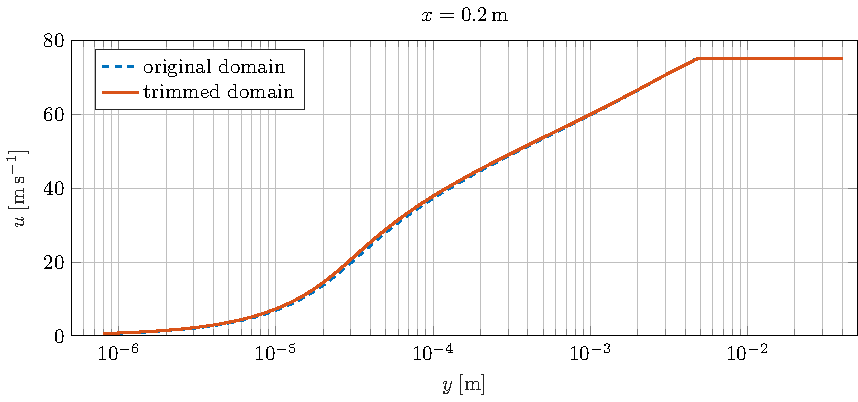
\includegraphics[width=13.5cm]{Results/ux2.pdf}
\caption{Graph of $x$ component of velocity field along the $x=0.2$ line from both original domain and the trimmed one.}
\label{fig::ux2}
\end{figure}

\begin{figure}[h]
\centering
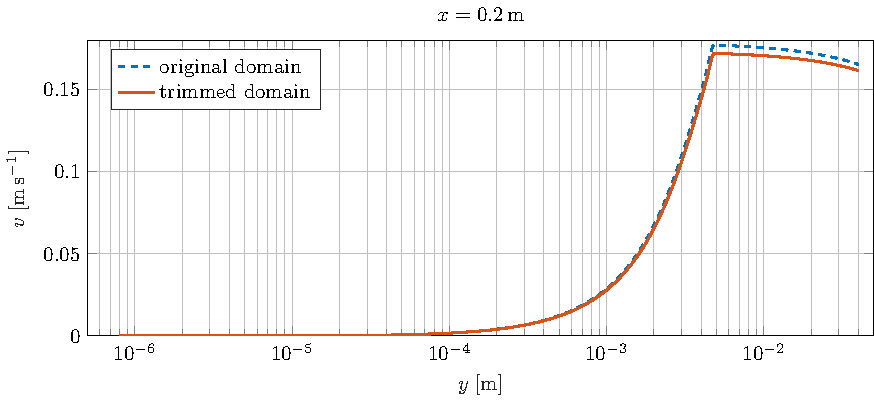
\includegraphics[width=13.5cm]{Results/uy2.pdf}
\caption{Graph of $y$ component of velocity field along the $x=0.2$ line from both original domain and the trimmed one.}
\label{fig::uy2}
\end{figure}

\begin{figure}
\centering
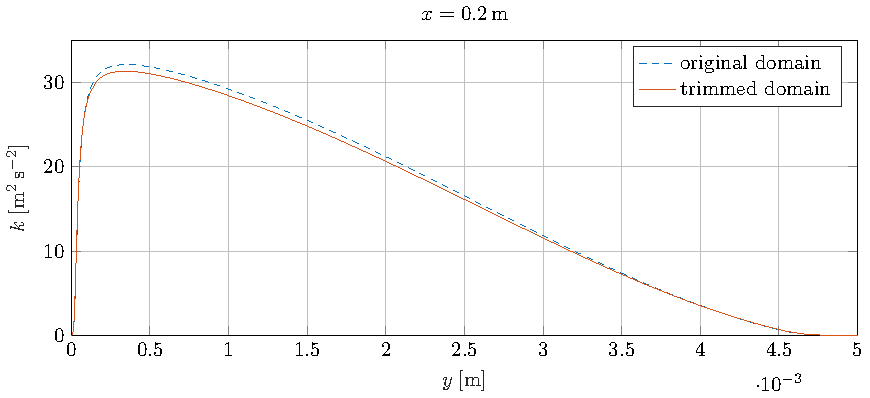
\includegraphics[width=14cm]{Results/k2.pdf}
\caption{Graph of turbulent kinetic energy field along the $x=0.2$ line from both original domain and the trimmed one.}
\label{fig::k2}
\end{figure}

\begin{figure}
\centering
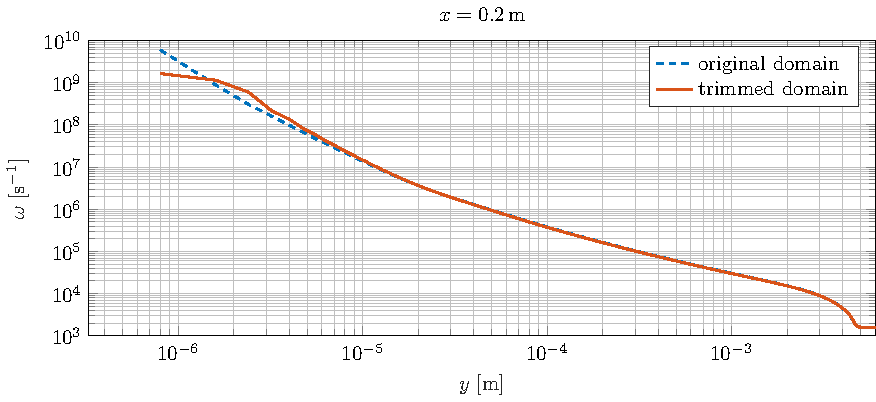
\includegraphics[width=14cm]{Results/omega2.pdf}
\caption{Graph of specific dissipation rate field along the $x=0.2$ line from both original domain and the trimmed one.}
\label{fig::omega2}
\end{figure}

\begin{figure}
\centering
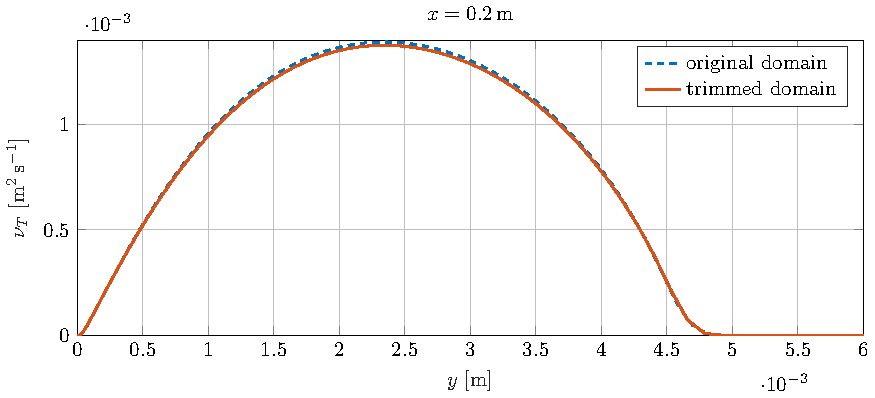
\includegraphics[width=14cm]{Results/nut2.pdf}
\caption{Graph of turbulent viscosity field along the $x=0.2$ line from both original domain and the trimmed one.}
\label{fig::nut2}
\end{figure}

\begin{figure}
\centering
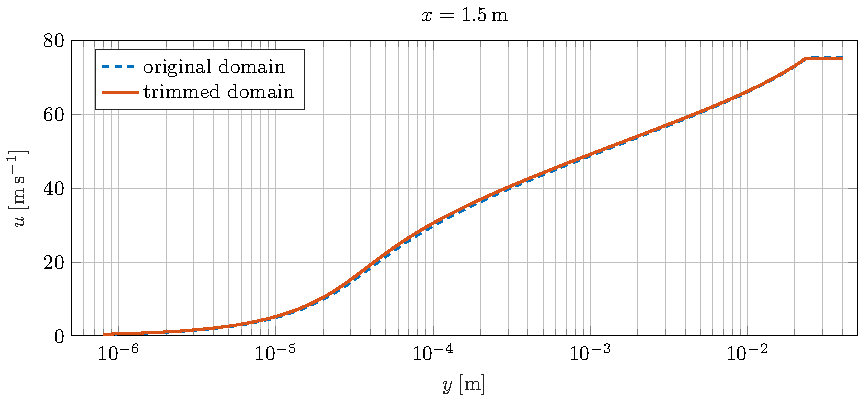
\includegraphics[width=14cm]{Results/ux15.pdf}
\caption{Graph of $x$ component of velocity field along the $x=1.5$ line from both original domain and the trimmed one.}
\label{fig::ux15}
\end{figure}

\begin{figure}
\centering
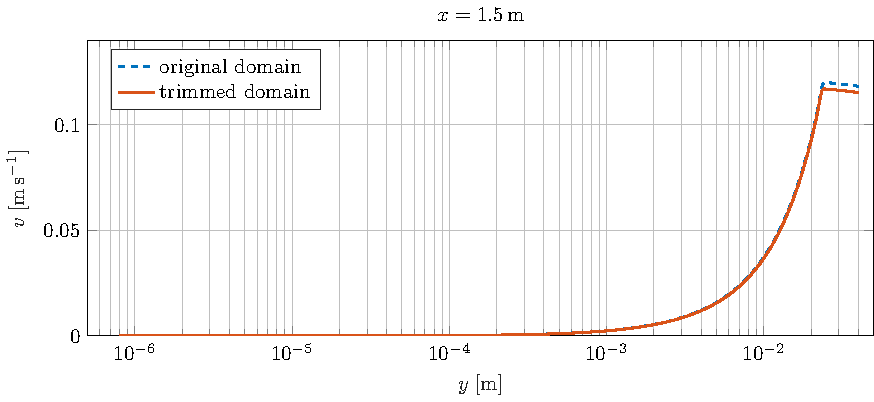
\includegraphics[width=14cm]{Results/uy15.pdf}
\caption{Graph of $y$ component of velocity field along the $x=1.5$ line from both original domain and the trimmed one.}
\label{fig::uy15}
\end{figure}

\begin{figure}
\centering
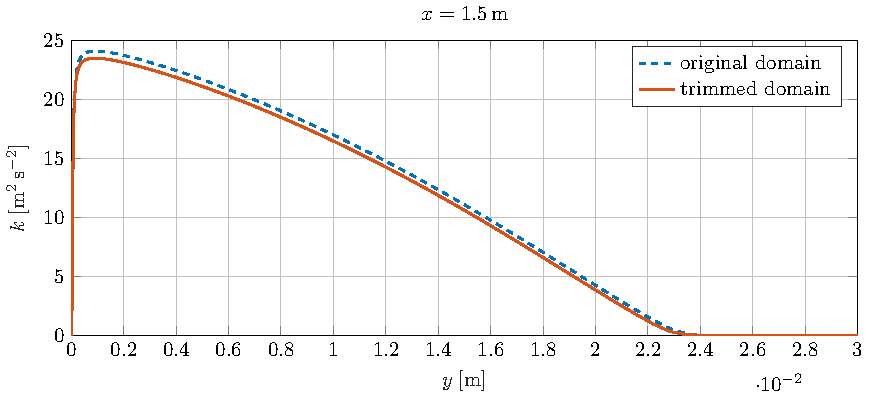
\includegraphics[width=14cm]{Results/k15.pdf}
\caption{Graph of turbulent kinetic energy field along the $x=1.5$ line from both original domain and the trimmed one.}
\label{fig::k15}
\end{figure}

\begin{figure}
\centering
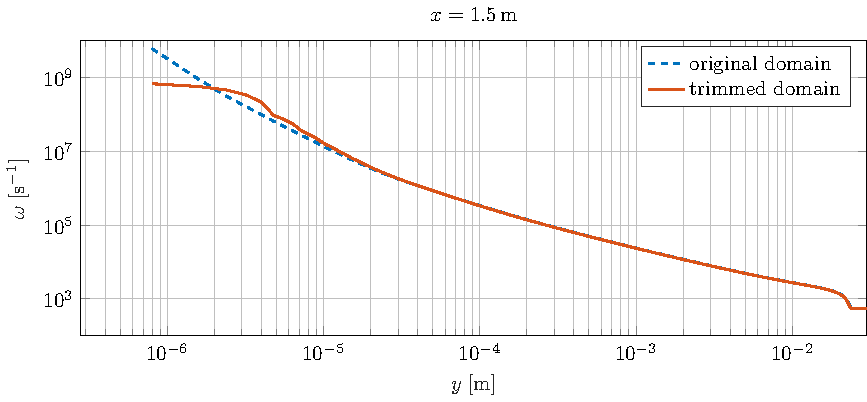
\includegraphics[width=14cm]{Results/omega15.pdf}
\caption{Graph of specific dissipation rate field along the $x=1.5$ line from both original domain and the trimmed one.}
\label{fig::omega15}
\end{figure}

\begin{figure}
\centering
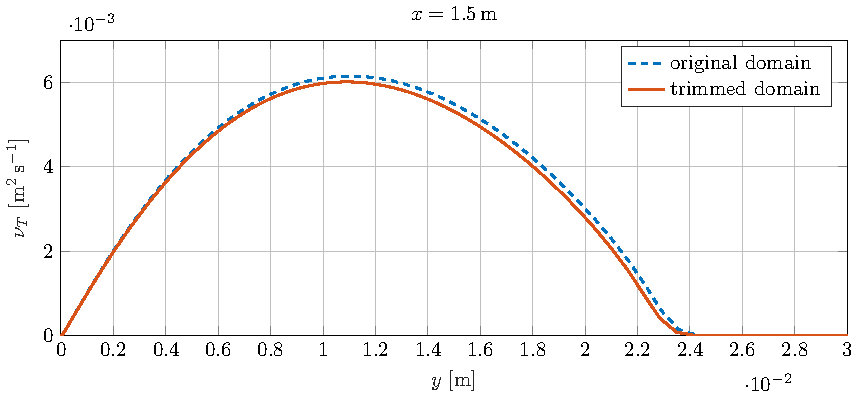
\includegraphics[width=14cm]{Results/nut15.pdf}
\caption{Graph of turbulent viscosity field along the $x=1.5$ line from both original domain and the trimmed one.}
\label{fig::nut15}
\end{figure}

    \chapter{Conclusions}
        Both simulations achieved very similar results differing very slightly (relative differences in field quantities were \SI{2}{\percent} at most on both of sampled lines). Those differences can be attributed mostly to two factors:
        \begin{itemize}
            \item Different mesh resolutions in  both simulations. 
            Each mesh was graded in the direction of the plates wall in order to achieve correct $y^+$ value (around \num{0,05} in case of original domain and \num{0.68} in the latter one), however mesh created for the second simulation is noticeably coarser.
            The reasoning behind this was to increase convergence rate by limiting high values of $\omega$ that can arise very close to the viscous wall.
            Nevertheless both meshes have adequate resolution to represent physical phenomena that arise in that type of flow.
            \item In the boundary layer region sampling points were separated by logarithmically rising intervals in order to account for sharply changing turbulent quantities. Sampled data was then linearly interpolated in order to impose boundary conditions. This interpolation might have introduced slight error in the fields that was than convected along plates surface.
        \end{itemize}

        In conclusion, goals that ware stated in the begging of this work were achieved. Author learned basic usage of \oFoam along with some other advanced practices i.e. tweaking linear solver settings or utilising advanced time and space varying boundary conditions.

        In the same time, this work has proven that \oFoam can be used as a tool for validation of various CFD models against experiments. Sampled data from those experiments can be used as boundary conditions in order to observe flow behaviour and assert validity of chosen model.
    
    \appendix

    \bibliography{Literature/bibfile}
\end{document} 
